\documentclass[11pt]{article}
\usepackage[utf8]{inputenc}
\usepackage[a4paper,margin=0.85in]{geometry}
\usepackage{amsmath,amsfonts,amssymb,amsthm}
\usepackage{enumitem}
\usepackage{parskip}
\usepackage{hyperref}
\usepackage{xcolor}
\usepackage{fancyhdr}
\usepackage{tikz}
\usepackage{graphicx}
\usepackage{eso-pic}
\usepackage{titlesec}
\usepackage{listings}

\graphicspath{{../}}

\definecolor{kcpc-text}{RGB}{20,20,20}
\definecolor{kcpc-muted}{RGB}{90,90,90}
\definecolor{kcpc-red}{RGB}{176,0,0}

\pagestyle{fancy}
\fancyhf{}
\lhead{\textcolor{kcpc-text}{\small\bfseries Solutions}}
\rhead{\textcolor{kcpc-muted}{\small Week 4}}
\cfoot{\textcolor{kcpc-muted}{\small KCPC}}
\renewcommand{\headrulewidth}{0.4pt}
\renewcommand{\headrule}{\hbox to\headwidth{\color{kcpc-red}\leaders\hrule height \headrulewidth\hfill}}
\renewcommand{\footrulewidth}{0pt}
\setlength{\headheight}{28pt}

\AddToShipoutPictureBG{%
    \begin{tikzpicture}[remember picture,overlay]
        \node[opacity=0.035, at=(current page.center)]
        {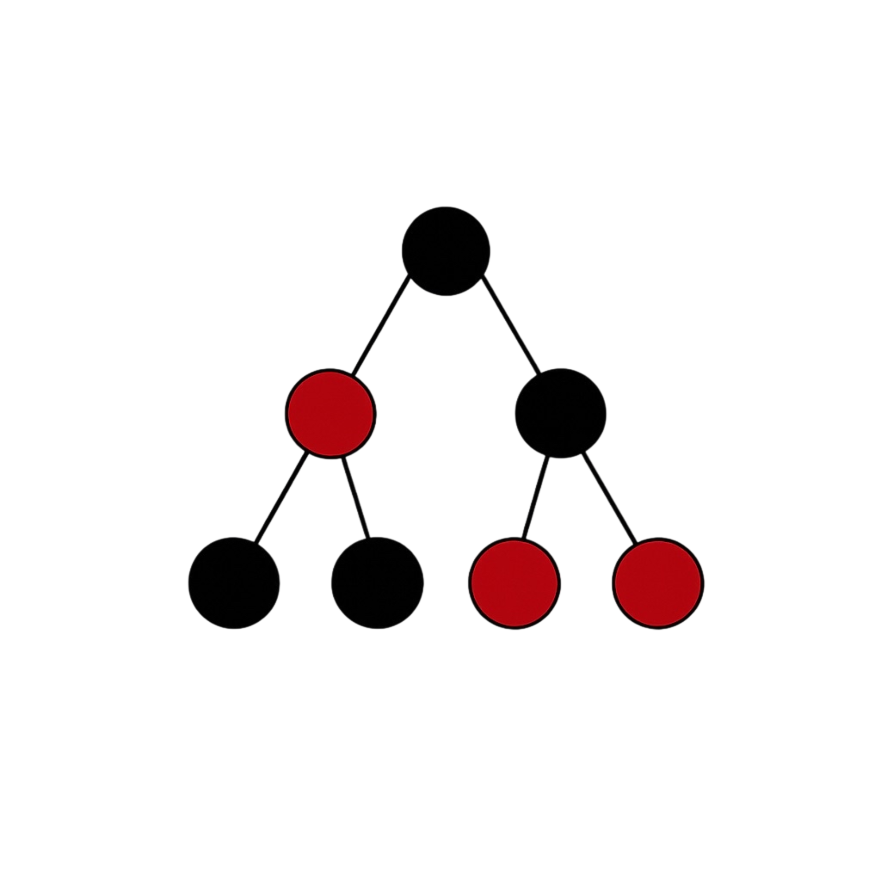
\includegraphics[width=0.38\paperwidth]{kcpc-logo.png}};
    \end{tikzpicture}%
}

\titleformat{\section}{\large\bfseries\color{kcpc-red}}{\thesection}{1em}{}

\newcommand{\insight}[1]{\par\medskip\noindent\textbf{Key insight:} #1\par\smallskip}

\lstset{
    basicstyle=\ttfamily\footnotesize,
    keywordstyle=\bfseries\color{kcpc-red},
    commentstyle=\itshape\color{kcpc-muted},
    breaklines=true,
    columns=fullflexible,
    keepspaces=true,
    frame=single,
    rulecolor=\color{kcpc-muted},
    showstringspaces=false
}

\hypersetup{
    colorlinks=true,
    linkcolor=kcpc-red,
    urlcolor=kcpc-red
}

\title{KCPC Week 4 Solutions\\Introduction to Graphs: Traversals, Structure, and Modelling}
\author{}
\date{}

\begin{document}

\maketitle
\thispagestyle{fancy}

\noindent
These official solutions accompany all 11 problems on the Workshop 4 problem sheet (Warm-Up Exercises, Core Practice Exercises, and Extended Homework). Every problem includes the underlying structural insight, a proof of correctness, complexity bounds, alternative approaches, and complete implementations in both \textbf{C++17} and \textbf{Python 3}.

% ============================================================
\section{Warm-Up Exercises (Foundational Traversals)}
% ============================================================

\subsection{Building Roads (\href{https://cses.fi/problemset/task/1666}{CSES 1666})}

\insight{Adding a single edge between two vertices in different connected components merges those two components into one, reducing the total number of connected components by at most $1$. Therefore, connecting $C$ components requires at least---and at most---$C - 1$ new edges.}

\textbf{Thought Process \& Proof:}
\begin{enumerate}
    \item Model the cities and bidirectional roads as an undirected graph $G = (V, E)$ with $|V| = n$ and $|E| = m$.
    \item Reachability in an undirected graph is an equivalence relation that partitions $V$ into $C$ disjoint \textbf{connected components}.
    \item Iterate $i$ from $1$ to $n$. Whenever city $i$ has not yet been visited, record $i$ as the representative $r_k$ of a new component and launch a DFS or BFS from $i$ to mark every city in that component as visited.
    \item Once all $C$ representatives $r_1, r_2, \dots, r_C$ are collected, adding the $C - 1$ edges $(r_1, r_2), (r_2, r_3), \dots, (r_{C-1}, r_C)$ (or connecting $r_1$ to every $r_k$ for $k \ge 2$) forms a spanning tree over the components, making the entire graph connected in the minimum possible $C - 1$ roads.
\end{enumerate}

\textbf{Alternative Approach:} Maintain a Disjoint Set Union (DSU / Union-Find) structure while reading the $m$ edges, then collect all vertices with $\texttt{parent}[i] = i$ as component representatives in $O((n + m)\alpha(n))$ time.

\textbf{Complexity:} Time $O(n + m)$, Auxiliary Space $O(n + m)$.

\textbf{C++17 Solution:}
\begin{lstlisting}[language=C++]
#include <iostream>
#include <vector>
using namespace std;

int main() {
    ios::sync_with_stdio(false);
    cin.tie(nullptr);

    int n, m;
    cin >> n >> m;
    vector<vector<int>> g(n + 1);
    for (int i = 0; i < m; ++i) {
        int u, v;
        cin >> u >> v;
        g[u].push_back(v);
        g[v].push_back(u);
    }

    vector<bool> vis(n + 1, false);
    vector<int> reps;

    for (int i = 1; i <= n; ++i) {
        if (!vis[i]) {
            reps.push_back(i);
            vector<int> st = {i};
            vis[i] = true;
            while (!st.empty()) {
                int v = st.back();
                st.pop_back();
                for (int u : g[v]) {
                    if (!vis[u]) {
                        vis[u] = true;
                        st.push_back(u);
                    }
                }
            }
        }
    }

    cout << (int)reps.size() - 1 << "\n";
    for (size_t i = 1; i < reps.size(); ++i) {
        cout << reps[i - 1] << " " << reps[i] << "\n";
    }
    return 0;
}
\end{lstlisting}

\textbf{Python 3 Solution:}
\begin{lstlisting}[language=Python]
import sys

def solve():
    input = sys.stdin.readline
    n, m = map(int, input().split())
    g = [[] for _ in range(n + 1)]
    for _ in range(m):
        u, v = map(int, input().split())
        g[u].append(v)
        g[v].append(u)

    vis = [False] * (n + 1)
    reps = []

    for i in range(1, n + 1):
        if not vis[i]:
            reps.append(i)
            stack = [i]
            vis[i] = True
            while stack:
                v = stack.pop()
                for u in g[v]:
                    if not vis[u]:
                        vis[u] = True
                        stack.append(u)

    out = [str(len(reps) - 1)]
    for i in range(1, len(reps)):
        out.append(f"{reps[i - 1]} {reps[i]}")
    print("\n".join(out))

if __name__ == "__main__":
    solve()
\end{lstlisting}

% ------------------------------------------------------------
\subsection{Message Route (\href{https://cses.fi/problemset/task/1667}{CSES 1667})}

\insight{Breadth-First Search visits vertices in non-decreasing order of distance from the source. Recording the discovering neighbour $\texttt{parent}[u] = v$ when $u$ is first enqueued implicitly builds a shortest-path tree.}

\textbf{Thought Process \& Proof:}
\begin{enumerate}
    \item In an unweighted graph, the minimum number of computers on a route from $1$ to $n$ equals $1 + \text{dist}(1, n)$, where $\text{dist}(1, n)$ is the minimum number of edges.
    \item Run BFS starting from source $1$ using a queue $q$ and an array $\texttt{parent}[1\dots n]$ initialised to $0$. Set $\texttt{parent}[1] = -1$ to mark the source as visited.
    \item By induction on distance layers, every reachable vertex $u$ is first discovered via a shortest path from $1$, and the edge $(\texttt{parent}[u], u)$ is the final edge on that shortest path.
    \item If $\texttt{parent}[n] = 0$ after the queue empties, computer $n$ lies in a different connected component, so we print \texttt{IMPOSSIBLE}. Otherwise, follow $v \leftarrow \texttt{parent}[v]$ from $n$ back to $1$ and reverse the list.
\end{enumerate}

\textbf{Complexity:} Time $O(n + m)$, Auxiliary Space $O(n + m)$.

\textbf{C++17 Solution:}
\begin{lstlisting}[language=C++]
#include <algorithm>
#include <iostream>
#include <queue>
#include <vector>
using namespace std;

int main() {
    ios::sync_with_stdio(false);
    cin.tie(nullptr);

    int n, m;
    cin >> n >> m;
    vector<vector<int>> g(n + 1);
    for (int i = 0; i < m; ++i) {
        int u, v;
        cin >> u >> v;
        g[u].push_back(v);
        g[v].push_back(u);
    }

    vector<int> parent(n + 1, 0);
    queue<int> q;
    q.push(1);
    parent[1] = -1;

    while (!q.empty()) {
        int v = q.front();
        q.pop();
        for (int u : g[v]) {
            if (parent[u] == 0) {
                parent[u] = v;
                q.push(u);
            }
        }
    }

    if (parent[n] == 0) {
        cout << "IMPOSSIBLE\n";
        return 0;
    }

    vector<int> path;
    for (int cur = n; cur != -1; cur = parent[cur]) {
        path.push_back(cur);
    }
    reverse(path.begin(), path.end());

    cout << path.size() << "\n";
    for (size_t i = 0; i < path.size(); ++i) {
        cout << path[i] << (i + 1 == path.size() ? '\n' : ' ');
    }
    return 0;
}
\end{lstlisting}

\textbf{Python 3 Solution:}
\begin{lstlisting}[language=Python]
from collections import deque
import sys

def solve():
    input = sys.stdin.readline
    n, m = map(int, input().split())
    g = [[] for _ in range(n + 1)]
    for _ in range(m):
        u, v = map(int, input().split())
        g[u].append(v)
        g[v].append(u)

    parent = [0] * (n + 1)
    parent[1] = -1
    q = deque([1])

    while q:
        v = q.popleft()
        if v == n:
            break
        for u in g[v]:
            if parent[u] == 0:
                parent[u] = v
                q.append(u)

    if parent[n] == 0:
        print("IMPOSSIBLE")
        return

    path = []
    cur = n
    while cur != -1:
        path.append(cur)
        cur = parent[cur]
    path.reverse()

    print(len(path))
    print(*(path))

if __name__ == "__main__":
    solve()
\end{lstlisting}

% ------------------------------------------------------------
\subsection{Round Trip (\href{https://cses.fi/problemset/task/1669}{CSES 1669})}

\insight{In an undirected simple graph, every non-tree edge encountered during Depth-First Search is a back-edge connecting the current vertex $v$ to an ancestor $u \neq \texttt{parent}[v]$. The tree path from $u$ to $v$ together with the back-edge $(v, u)$ forms a simple cycle of length $\ge 3$.}

\textbf{Thought Process \& Proof:}
\begin{enumerate}
    \item A round trip through at least three distinct cities is precisely a simple cycle in the undirected graph.
    \item Run DFS from each unvisited vertex $i \in \{1, \dots, n\}$. When exploring neighbours $u$ of $v$:
    \begin{itemize}
        \item Ignore the edge leading immediately back to $\texttt{parent}[v]$ (since traversing an undirected edge back and forth has length $2$ and is not a valid simple cycle).
        \item If $u$ is unvisited, set $\texttt{parent}[u] = v$ and recurse.
        \item If $u$ is already visited and $u \neq \texttt{parent}[v]$, then $u$ is an ancestor of $v$ in the DFS tree.
    \end{itemize}
    \item Reconstruct the cycle by starting with $u$, walking $x \leftarrow \texttt{parent}[x]$ from $v$ up to $u$, and ending at $u$. Because $u \neq \texttt{parent}[v]$, the path contains at least three distinct vertices.
\end{enumerate}

\textbf{Complexity:} Time $O(n + m)$, Auxiliary Space $O(n + m)$.

\textbf{C++17 Solution:}
\begin{lstlisting}[language=C++]
#include <iostream>
#include <vector>
using namespace std;

int n, m;
vector<vector<int>> g;
vector<int> parent_node;
vector<bool> vis;
int cyc_start = -1, cyc_end = -1;

bool dfs(int v, int p) {
    vis[v] = true;
    for (int u : g[v]) {
        if (u == p) continue;
        if (vis[u]) {
            cyc_end = v;
            cyc_start = u;
            return true;
        }
        parent_node[u] = v;
        if (dfs(u, v)) return true;
    }
    return false;
}

int main() {
    ios::sync_with_stdio(false);
    cin.tie(nullptr);

    cin >> n >> m;
    g.resize(n + 1);
    for (int i = 0; i < m; ++i) {
        int u, v;
        cin >> u >> v;
        g[u].push_back(v);
        g[v].push_back(u);
    }

    vis.assign(n + 1, false);
    parent_node.assign(n + 1, -1);

    for (int i = 1; i <= n; ++i) {
        if (!vis[i] && dfs(i, -1)) break;
    }

    if (cyc_start == -1) {
        cout << "IMPOSSIBLE\n";
        return 0;
    }

    vector<int> cycle = {cyc_start};
    for (int v = cyc_end; v != cyc_start; v = parent_node[v]) {
        cycle.push_back(v);
    }
    cycle.push_back(cyc_start);

    cout << cycle.size() << "\n";
    for (size_t i = 0; i < cycle.size(); ++i) {
        cout << cycle[i] << (i + 1 == cycle.size() ? '\n' : ' ');
    }
    return 0;
}
\end{lstlisting}

\textbf{Python 3 Solution:}
\begin{lstlisting}[language=Python]
import sys

def solve():
    sys.setrecursionlimit(300000)
    input = sys.stdin.readline
    n, m = map(int, input().split())
    g = [[] for _ in range(n + 1)]
    for _ in range(m):
        u, v = map(int, input().split())
        g[u].append(v)
        g[v].append(u)

    vis = [False] * (n + 1)
    parent = [0] * (n + 1)
    cyc_start, cyc_end = -1, -1

    # Iterative DFS with explicit neighbour-index stack avoids recursion limit overhead
    for i in range(1, n + 1):
        if vis[i]:
            continue
        vis[i] = True
        stack = [(i, 0)]
        found = False
        while stack and not found:
            v, idx = stack[-1]
            if idx < len(g[v]):
                u = g[v][idx]
                stack[-1] = (v, idx + 1)
                if u == parent[v]:
                    continue
                if vis[u]:
                    cyc_start, cyc_end = u, v
                    found = True
                    break
                vis[u] = True
                parent[u] = v
                stack.append((u, 0))
            else:
                stack.pop()
        if found:
            break

    if cyc_start == -1:
        print("IMPOSSIBLE")
        return

    cycle = [cyc_start]
    cur = cyc_end
    while cur != cyc_start:
        cycle.append(cur)
        cur = parent[cur]
    cycle.append(cyc_start)

    print(len(cycle))
    print(*(cycle))

if __name__ == "__main__":
    solve()
\end{lstlisting}

% ------------------------------------------------------------
\subsection{Building Teams (\href{https://cses.fi/problemset/task/1668}{CSES 1668})}

\insight{Dividing vertices into two conflict-free teams is equivalent to 2-colouring the graph (testing bipartiteness). Once one vertex in a connected component is assigned team $1$, the team of every other vertex in that component is uniquely forced.}

\textbf{Thought Process \& Proof:}
\begin{enumerate}
    \item Let $\texttt{col}[v] \in \{0, 1, 2\}$ denote the team of pupil $v$ ($0$ means unassigned).
    \item Iterate $i$ from $1$ to $n$. If $\texttt{col}[i] = 0$, set $\texttt{col}[i] = 1$ and run BFS (or DFS) to propagate colours across $i$'s connected component:
    \begin{itemize}
        \item For every edge $(v, u)$, $u$ cannot share $v$'s team, so $u$ is forced to take the opposite team $3 - \texttt{col}[v]$.
        \item If $\texttt{col}[u] = 0$, assign $\texttt{col}[u] = 3 - \texttt{col}[v]$ and push $u$.
        \item If $\texttt{col}[u] = \texttt{col}[v]$, we have discovered two adjacent vertices at the same distance parity from $i$, which forms an odd-length cycle. No valid 2-colouring exists, so we output \texttt{IMPOSSIBLE}.
    \end{itemize}
    \item If all components are processed without conflict, $\texttt{col}[1\dots n]$ is a valid bipartite partition.
\end{enumerate}

\textbf{Complexity:} Time $O(n + m)$, Auxiliary Space $O(n + m)$.

\textbf{C++17 Solution:}
\begin{lstlisting}[language=C++]
#include <iostream>
#include <queue>
#include <vector>
using namespace std;

int main() {
    ios::sync_with_stdio(false);
    cin.tie(nullptr);

    int n, m;
    cin >> n >> m;
    vector<vector<int>> g(n + 1);
    for (int i = 0; i < m; ++i) {
        int u, v;
        cin >> u >> v;
        g[u].push_back(v);
        g[v].push_back(u);
    }

    vector<int> col(n + 1, 0);
    queue<int> q;

    for (int i = 1; i <= n; ++i) {
        if (col[i] != 0) continue;
        col[i] = 1;
        q.push(i);
        while (!q.empty()) {
            int v = q.front();
            q.pop();
            for (int u : g[v]) {
                if (col[u] == 0) {
                    col[u] = 3 - col[v];
                    q.push(u);
                } else if (col[u] == col[v]) {
                    cout << "IMPOSSIBLE\n";
                    return 0;
                }
            }
        }
    }

    for (int i = 1; i <= n; ++i) {
        cout << col[i] << (i == n ? '\n' : ' ');
    }
    return 0;
}
\end{lstlisting}

\textbf{Python 3 Solution:}
\begin{lstlisting}[language=Python]
from collections import deque
import sys

def solve():
    input = sys.stdin.readline
    n, m = map(int, input().split())
    g = [[] for _ in range(n + 1)]
    for _ in range(m):
        u, v = map(int, input().split())
        g[u].append(v)
        g[v].append(u)

    col = [0] * (n + 1)
    for i in range(1, n + 1):
        if col[i] != 0:
            continue
        col[i] = 1
        q = deque([i])
        while q:
            v = q.popleft()
            next_col = 3 - col[v]
            for u in g[v]:
                if col[u] == 0:
                    col[u] = next_col
                    q.append(u)
                elif col[u] == col[v]:
                    print("IMPOSSIBLE")
                    return

    print(*(col[1:]))

if __name__ == "__main__":
    solve()
\end{lstlisting}

% ============================================================
\section{Core Practice Exercises (Structure, Trees, and DAGs)}
% ============================================================

\subsection{Badge (\href{https://codeforces.com/contest/1020/problem/B}{Codeforces 1020B})}

\insight{A directed graph in which every vertex has out-degree $1$ is a \emph{functional graph}. Every walk $a \to p_a \to p_{p_a} \to \dots$ on a finite functional graph must enter a directed cycle within at most $n$ steps. A vertex $v$ on the cycle returns $v$ itself, whereas a vertex $u$ outside the cycle returns the unique cycle vertex where its path first enters the cycle.}

\textbf{Thought Process \& Two Solution Strategies:}
\begin{enumerate}
    \item \textbf{Strategy 1 ($O(n^2)$ Direct Walk):} Since $n \le 1000$, for each starting student $a \in \{1, \dots, n\}$, we can simply walk $cur \leftarrow p_{cur}$ while marking visited students until we hit a student already visited in the current walk. This takes at most $n + 1$ steps per starting student, or $O(n^2)$ time overall.
    \item \textbf{Strategy 2 ($O(n)$ Cycle \& Tree Propagation):} What if $n = 2 \cdot 10^5$? In any functional graph, each component consists of one directed cycle $C$ plus trees directed into $C$.
    \begin{itemize}
        \item For any vertex $v \in C$, following $p$ goes around $C$ and returns to $v$ first, so $\text{ans}[v] = v$.
        \item For any vertex $u \notin C$, its path enters $C$ at some entry vertex $w \in C$ and then loops around $C$ back to $w$, so $\text{ans}[u] = w = \text{ans}[p_u]$.
    \end{itemize}
    Thus, we can identify all cycle vertices in $O(n)$ using 3-state DFS (or Kahn's in-degree peeling), set $\text{ans}[v] = v$ on cycles, and memoize $\text{ans}[u] = \text{ans}[p_u]$ outside cycles in $O(n)$ total time! Below we provide the $O(n^2)$ direct traversal in C++ and the $O(n)$ linear algorithm in Python so both techniques are illustrated.
\end{enumerate}

\textbf{Complexity:} Strategy 1: Time $O(n^2)$, Space $O(n)$. Strategy 2: Time $O(n)$, Space $O(n)$.

\textbf{C++17 Solution (Direct $O(n^2)$ Traversal):}
\begin{lstlisting}[language=C++]
#include <iostream>
#include <vector>
using namespace std;

int main() {
    ios::sync_with_stdio(false);
    cin.tie(nullptr);

    int n;
    cin >> n;
    vector<int> p(n + 1);
    for (int i = 1; i <= n; ++i) {
        cin >> p[i];
    }

    for (int start = 1; start <= n; ++start) {
        vector<bool> vis(n + 1, false);
        int cur = start;
        while (!vis[cur]) {
            vis[cur] = true;
            cur = p[cur];
        }
        cout << cur << (start == n ? '\n' : ' ');
    }
    return 0;
}
\end{lstlisting}

\textbf{Python 3 Solution (Optimal $O(n)$ Functional Graph Analysis):}
\begin{lstlisting}[language=Python]
import sys

def solve():
    input = sys.stdin.readline
    n = int(input())
    p = [0] + list(map(int, input().split()))

    ans = [0] * (n + 1)
    state = [0] * (n + 1)  # 0 = unvisited, 1 = on current path, 2 = resolved

    for i in range(1, n + 1):
        if state[i] != 0:
            continue
        path = []
        cur = i
        while state[cur] == 0:
            state[cur] = 1
            path.append(cur)
            cur = p[cur]

        if state[cur] == 1:
            # cur is the entry of a newly discovered cycle
            in_cycle = False
            for node in path:
                if node == cur:
                    in_cycle = True
                if in_cycle:
                    ans[node] = node
                    state[node] = 2

        # Resolve remaining prefix nodes in reverse order
        for node in reversed(path):
            if state[node] != 2:
                ans[node] = ans[p[node]]
                state[node] = 2

    print(*(ans[1:]))

if __name__ == "__main__":
    solve()
\end{lstlisting}

% ------------------------------------------------------------
\subsection{Cyclic Components (\href{https://codeforces.com/problemset/problem/977/E}{Codeforces 977E})}

\insight{A connected component in a finite undirected simple graph is a simple cycle if and only if every vertex in the component has degree exactly $2$.}

\textbf{Thought Process \& Proof:}
\begin{itemize}
    \item \textbf{Necessity ($\implies$):} In any simple cycle $(v_1, v_2, \dots, v_k, v_1)$ with $k \ge 3$, each vertex $v_i$ is adjacent only to its predecessor and successor, so $\deg(v_i) = 2$ for all $i$.
    \item \textbf{Sufficiency ($\Longleftarrow$):} Suppose $C$ is a connected component in which $\deg(v) = 2$ for every $v \in C$. Because the graph has no self-loops or multiple edges, $C$ must have $|C| \ge 3$. Start at any $v_1 \in C$ and walk along unvisited edges. Each time we enter a new vertex $v_i$, it has degree $2$ (one edge used to enter, one remaining edge to leave), so the walk can never get stuck at any vertex other than $v_1$. Since $C$ is finite, the walk must eventually return to $v_1$, forming a simple cycle $S \subseteq C$. Every vertex on $S$ already has both of its incident edges inside $S$; because $C$ is connected, no other vertices can exist in $C \setminus S$, so $C = S$ is a simple cycle.
\end{itemize}
Thus we simply traverse each connected component via BFS/DFS and check whether $\deg(v) = 2$ holds for all vertices $v$ in that component.

\textbf{Complexity:} Time $O(n + m)$, Auxiliary Space $O(n + m)$.

\textbf{C++17 Solution:}
\begin{lstlisting}[language=C++]
#include <iostream>
#include <vector>
using namespace std;

int main() {
    ios::sync_with_stdio(false);
    cin.tie(nullptr);

    int n, m;
    cin >> n >> m;
    vector<vector<int>> g(n + 1);
    for (int i = 0; i < m; ++i) {
        int u, v;
        cin >> u >> v;
        g[u].push_back(v);
        g[v].push_back(u);
    }

    vector<bool> vis(n + 1, false);
    int cyclic_components = 0;

    for (int i = 1; i <= n; ++i) {
        if (vis[i]) continue;
        bool all_deg_two = true;
        vector<int> st = {i};
        vis[i] = true;
        while (!st.empty()) {
            int v = st.back();
            st.pop_back();
            if (g[v].size() != 2) {
                all_deg_two = false;
            }
            for (int u : g[v]) {
                if (!vis[u]) {
                    vis[u] = true;
                    st.push_back(u);
                }
            }
        }
        if (all_deg_two) {
            ++cyclic_components;
        }
    }

    cout << cyclic_components << "\n";
    return 0;
}
\end{lstlisting}

\textbf{Python 3 Solution:}
\begin{lstlisting}[language=Python]
import sys

def solve():
    input = sys.stdin.readline
    n, m = map(int, input().split())
    g = [[] for _ in range(n + 1)]
    for _ in range(m):
        u, v = map(int, input().split())
        g[u].append(v)
        g[v].append(u)

    vis = [False] * (n + 1)
    cyclic_components = 0

    for i in range(1, n + 1):
        if vis[i]:
            continue
        all_deg_two = True
        stack = [i]
        vis[i] = True
        while stack:
            v = stack.pop()
            if len(g[v]) != 2:
                all_deg_two = False
            for u in g[v]:
                if not vis[u]:
                    vis[u] = True
                    stack.append(u)
        if all_deg_two:
            cyclic_components += 1

    print(cyclic_components)

if __name__ == "__main__":
    solve()
\end{lstlisting}

% ------------------------------------------------------------
\subsection{DAG Number of Routes / Game Routes (\href{https://cses.fi/problemset/task/1681}{CSES 1681})}

\insight{Because a Directed Acyclic Graph (DAG) contains no directed cycles, its vertices admit a topological ordering $v_1, v_2, \dots, v_n$ where every edge $u \to v$ satisfies $\text{pos}(u) < \text{pos}(v)$. Processing vertices in topological order guarantees that when we reach $u$, the total number of paths $\text{dp}[u]$ from $1$ to $u$ is already completely computed.}

\textbf{Thought Process \& Proof:}
\begin{enumerate}
    \item Every valid route from $1$ to $v$ ($v \neq 1$) must traverse some final edge $u \to v$, preceded by a valid route from $1$ to $u$. Hence:
    \[ \text{dp}[1] = 1, \qquad \text{dp}[v] = \sum_{(u \to v) \in E} \text{dp}[u] \pmod{10^9 + 7}. \]
    \item Using \textbf{Kahn's Algorithm}, compute the in-degree $\texttt{indeg}[v]$ of every vertex and push all vertices with $\texttt{indeg}[v] = 0$ into a queue.
    \item Repeatedly pop $u$ from the queue and for each outgoing edge $u \to v$:
    \begin{itemize}
        \item Add $\text{dp}[u]$ to $\text{dp}[v]$ modulo $10^9 + 7$.
        \item Decrement $\texttt{indeg}[v]$, and if $\texttt{indeg}[v] = 0$, push $v$ into the queue.
    \end{itemize}
    \item By induction on the topological index, $\text{dp}[n]$ holds the exact number of routes from $1$ to $n$ modulo $10^9 + 7$.
\end{enumerate}

\textbf{Complexity:} Time $O(n + m)$, Auxiliary Space $O(n + m)$.

\textbf{C++17 Solution:}
\begin{lstlisting}[language=C++]
#include <iostream>
#include <queue>
#include <vector>
using namespace std;

int main() {
    ios::sync_with_stdio(false);
    cin.tie(nullptr);

    constexpr int MOD = 1000000007;
    int n, m;
    cin >> n >> m;
    vector<vector<int>> g(n + 1);
    vector<int> indeg(n + 1, 0);
    for (int i = 0; i < m; ++i) {
        int u, v;
        cin >> u >> v;
        g[u].push_back(v);
        ++indeg[v];
    }

    queue<int> q;
    for (int i = 1; i <= n; ++i) {
        if (indeg[i] == 0) q.push(i);
    }

    vector<int> dp(n + 1, 0);
    dp[1] = 1;

    while (!q.empty()) {
        int u = q.front();
        q.pop();
        for (int v : g[u]) {
            dp[v] = (dp[v] + dp[u]) % MOD;
            if (--indeg[v] == 0) {
                q.push(v);
            }
        }
    }

    cout << dp[n] << "\n";
    return 0;
}
\end{lstlisting}

\textbf{Python 3 Solution:}
\begin{lstlisting}[language=Python]
from collections import deque
import sys

def solve():
    input = sys.stdin.readline
    MOD = 10**9 + 7
    n, m = map(int, input().split())
    g = [[] for _ in range(n + 1)]
    indeg = [0] * (n + 1)
    for _ in range(m):
        u, v = map(int, input().split())
        g[u].append(v)
        indeg[v] += 1

    q = deque(i for i in range(1, n + 1) if indeg[i] == 0)
    dp = [0] * (n + 1)
    dp[1] = 1

    while q:
        u = q.popleft()
        du = dp[u]
        for v in g[u]:
            if du:
                dp[v] = (dp[v] + du) % MOD
            indeg[v] -= 1
            if indeg[v] == 0:
                q.append(v)

    print(dp[n])

if __name__ == "__main__":
    solve()
\end{lstlisting}

% ------------------------------------------------------------
\subsection{Longest Path (\href{https://atcoder.jp/contests/dp/tasks/dp_g}{AtCoder DP Contest G})}

\insight{Although finding the longest simple path in a general graph is NP-hard, on a DAG there are no cycles, so optimal substructure holds without tracking visited sets: the longest path starting at $u$ is $0$ if $u$ is a sink, or $\max_{u \to v} (1 + \text{dp}[v])$.}

\textbf{Thought Process \& Proof:}
\begin{enumerate}
    \item We can compute $\text{dp}$ either \textbf{top-down} (memoized DFS, where $\text{dp}[u] = \max_{u \to v}(1 + \text{dp}[v])$) or \textbf{bottom-up} (using Kahn's topological sort, where $\text{dp}[v]$ is the longest path \emph{ending} at $v$, updated via $\text{dp}[v] = \max(\text{dp}[v], \text{dp}[u] + 1)$ along each edge $u \to v$).
    \item Either way, each vertex and directed edge is processed a constant number of times, and the global maximum $\max_{1 \le i \le N} \text{dp}[i]$ gives the length of the longest directed path in $G$.
\end{enumerate}

\textbf{Complexity:} Time $O(N + M)$, Auxiliary Space $O(N + M)$.

\textbf{C++17 Solution (Memoized DFS):}
\begin{lstlisting}[language=C++]
#include <algorithm>
#include <iostream>
#include <vector>
using namespace std;

int n, m;
vector<vector<int>> g;
vector<int> memo;

int dfs(int u) {
    if (memo[u] != -1) return memo[u];
    int best = 0;
    for (int v : g[u]) {
        best = max(best, 1 + dfs(v));
    }
    return memo[u] = best;
}

int main() {
    ios::sync_with_stdio(false);
    cin.tie(nullptr);

    cin >> n >> m;
    g.resize(n + 1);
    for (int i = 0; i < m; ++i) {
        int u, v;
        cin >> u >> v;
        g[u].push_back(v);
    }

    memo.assign(n + 1, -1);
    int ans = 0;
    for (int i = 1; i <= n; ++i) {
        ans = max(ans, dfs(i));
    }
    cout << ans << "\n";
    return 0;
}
\end{lstlisting}

\textbf{Python 3 Solution (Kahn's Topological DP):}
\begin{lstlisting}[language=Python]
from collections import deque
import sys

def solve():
    input = sys.stdin.readline
    n, m = map(int, input().split())
    g = [[] for _ in range(n + 1)]
    indeg = [0] * (n + 1)
    for _ in range(m):
        u, v = map(int, input().split())
        g[u].append(v)
        indeg[v] += 1

    q = deque(i for i in range(1, n + 1) if indeg[i] == 0)
    dp = [0] * (n + 1)

    while q:
        u = q.popleft()
        du = dp[u] + 1
        for v in g[u]:
            if du > dp[v]:
                dp[v] = du
            indeg[v] -= 1
            if indeg[v] == 0:
                q.append(v)

    print(max(dp))

if __name__ == "__main__":
    solve()
\end{lstlisting}

% ------------------------------------------------------------
\subsection{Tree Diameter (\href{https://cses.fi/problemset/task/1131}{CSES 1131})}

\insight{In any tree, a node $u$ at maximum distance from an arbitrary starting node $r$ is guaranteed to be an endpoint of a diameter (longest simple path). A second traversal from $u$ finds the other endpoint $v$ and the diameter $d(u, v)$.}

\textbf{Proof of the Two-BFS Theorem:}
Let $P_{xy}$ be a longest path in the tree $T$, so $d(x, y) = D$ is the diameter, and let $u$ be a vertex maximising $d(r, u)$ from an arbitrary root $r$. We prove that $u$ can replace one endpoint of $P_{xy}$, i.e., $\max(d(u, x), d(u, y)) = D$.
\begin{itemize}
    \item Because $T$ is a tree, there is a unique projection vertex $w \in P_{xy}$ closest to $r$ (the unique junction where the path from $r$ meets $P_{xy}$), so $d(r, x) = d(r, w) + d(w, x)$ and $d(r, y) = d(r, w) + d(w, y)$.
    \item Let $z$ be the last vertex shared by the unique path from $r$ to $u$ and the union of paths from $r$ to $P_{xy}$.
    \item If $z$ lies on the segment between $r$ and $w$, then the path from $u$ to $x$ passes through $z$ and $w$, giving:
    \[ d(u, x) = d(u, z) + d(z, w) + d(w, x). \]
    Since $d(r, u) \ge d(r, y)$ by choice of $u$, we have $d(r, z) + d(z, u) \ge d(r, z) + d(z, w) + d(w, y) \implies d(u, z) \ge d(z, w) + d(w, y) \ge d(w, y)$. Substituting this in yields $d(u, x) \ge d(w, y) + d(w, x) = d(x, y) = D$.
    \item Otherwise, $z$ lies on $P_{xy}$ (say between $w$ and $y$). Then $d(r, u) \ge d(r, y) \implies d(z, u) \ge d(z, y)$, so the path from $x$ to $u$ via $z$ has length $d(x, z) + d(z, u) \ge d(x, z) + d(z, y) = D$.
\end{itemize}
In every case $\max(d(u, x), d(u, y)) = D$, so a second BFS/DFS from $u$ finds a node $v$ at distance $D$.

\textbf{Complexity:} Time $O(n)$, Auxiliary Space $O(n)$.

\textbf{C++17 Solution:}
\begin{lstlisting}[language=C++]
#include <iostream>
#include <queue>
#include <utility>
#include <vector>
using namespace std;

pair<int, int> farthest_node(int start, int n, const vector<vector<int>>& g) {
    vector<int> dist(n + 1, -1);
    queue<int> q;
    q.push(start);
    dist[start] = 0;
    int best_node = start;

    while (!q.empty()) {
        int v = q.front();
        q.pop();
        if (dist[v] > dist[best_node]) {
            best_node = v;
        }
        for (int u : g[v]) {
            if (dist[u] == -1) {
                dist[u] = dist[v] + 1;
                q.push(u);
            }
        }
    }
    return {best_node, dist[best_node]};
}

int main() {
    ios::sync_with_stdio(false);
    cin.tie(nullptr);

    int n;
    cin >> n;
    vector<vector<int>> g(n + 1);
    for (int i = 0; i < n - 1; ++i) {
        int u, v;
        cin >> u >> v;
        g[u].push_back(v);
        g[v].push_back(u);
    }

    auto [u, _] = farthest_node(1, n, g);
    auto [v, diameter] = farthest_node(u, n, g);
    cout << diameter << "\n";
    return 0;
}
\end{lstlisting}

\textbf{Python 3 Solution:}
\begin{lstlisting}[language=Python]
from collections import deque
import sys

def bfs(start, n, g):
    dist = [-1] * (n + 1)
    dist[start] = 0
    q = deque([start])
    last = start
    while q:
        v = q.popleft()
        last = v
        dv = dist[v] + 1
        for u in g[v]:
            if dist[u] == -1:
                dist[u] = dv
                q.append(u)
    return last, dist[last]

def solve():
    input = sys.stdin.readline
    n = int(input())
    g = [[] for _ in range(n + 1)]
    for _ in range(n - 1):
        u, v = map(int, input().split())
        g[u].append(v)
        g[v].append(u)

    u, _ = bfs(1, n, g)
    _, diameter = bfs(u, n, g)
    print(diameter)

if __name__ == "__main__":
    solve()
\end{lstlisting}

% ============================================================
\section{Extended Homework (Advanced Graph Modelling)}
% ============================================================

\subsection{Rudolf and Subway (\href{https://codeforces.com/contest/1941/problem/G}{Codeforces 1941G})}

\insight{Instead of adding $O(k^2)$ direct edges between $k$ stations on the same subway line, introduce an auxiliary vertex $L_c$ for each colour $c$ and connect every station on line $c$ to $L_c$. Riding line $c$ from station $u$ to station $v$ becomes a $2$-edge path $u \to L_c \to v$ in an unweighted bipartite graph.}

\textbf{Thought Process \& Proof:}
\begin{enumerate}
    \item Notice that the problem assumes each colour $c$ forms a single connected subway line. Travelling between any two stations $u$ and $v$ that both touch edges of colour $c$ costs $1$ ticket on line $c$.
    \item Construct an unweighted bipartite graph $H$:
    \begin{itemize}
        \item Left partition: station vertices $1, 2, \dots, n$.
        \item Right partition: one auxiliary colour vertex $L_c$ for each distinct colour $c$ appearing in the test case (assigning IDs $n + 1, n + 2, \dots, n + K$).
        \item For each input track $(u, v, c)$, add undirected edges $\{u, L_c\}$ and $\{v, L_c\}$.
    \end{itemize}
    \item Any path in $H$ alternates strictly between station vertices and colour vertices:
    \[ b = s_0 \to L_{c_1} \to s_1 \to L_{c_2} \to \dots \to L_{c_t} \to s_t = e. \]
    This sequence uses $t$ subway lines and has $2t$ edges in $H$. Therefore, the minimum number of subway lines from $b$ to $e$ is exactly $\frac{1}{2}\text{dist}_H(b, e)$, which we compute via standard BFS!
\end{enumerate}

\textbf{Complexity:} Time $O(n + m)$ per test case, Auxiliary Space $O(n + m)$.

\textbf{C++17 Solution:}
\begin{lstlisting}[language=C++]
#include <algorithm>
#include <iostream>
#include <queue>
#include <unordered_map>
#include <vector>
using namespace std;

void solve_case() {
    int n, m;
    cin >> n >> m;

    unordered_map<int, int> color_id;
    color_id.reserve(2 * m);
    int next_id = n + 1;

    struct RawEdge { int u, v, c_node; };
    vector<RawEdge> edges;
    edges.reserve(m);

    for (int i = 0; i < m; ++i) {
        int u, v, c;
        cin >> u >> v >> c;
        auto it = color_id.find(c);
        int c_node;
        if (it == color_id.end()) {
            c_node = next_id++;
            color_id[c] = c_node;
        } else {
            c_node = it->second;
        }
        edges.push_back({u, v, c_node});
    }

    int b, e;
    cin >> b >> e;
    if (b == e) {
        cout << 0 << "\n";
        return;
    }

    int total_nodes = next_id;
    vector<vector<int>> g(total_nodes);
    for (const auto& ed : edges) {
        g[ed.u].push_back(ed.c_node);
        g[ed.c_node].push_back(ed.u);
        g[ed.v].push_back(ed.c_node);
        g[ed.c_node].push_back(ed.v);
    }

    vector<int> dist(total_nodes, -1);
    queue<int> q;
    q.push(b);
    dist[b] = 0;

    while (!q.empty()) {
        int v = q.front();
        q.pop();
        if (v == e) break;
        for (int u : g[v]) {
            if (dist[u] == -1) {
                dist[u] = dist[v] + 1;
                q.push(u);
            }
        }
    }

    cout << dist[e] / 2 << "\n";
}

int main() {
    ios::sync_with_stdio(false);
    cin.tie(nullptr);

    int t;
    cin >> t;
    while (t--) {
        solve_case();
    }
    return 0;
}
\end{lstlisting}

\textbf{Python 3 Solution:}
\begin{lstlisting}[language=Python]
from collections import deque
import sys

def solve():
    input = sys.stdin.readline
    t = int(input())
    out = []
    for _ in range(t):
        n, m = map(int, input().split())
        color_id = {}
        next_id = n + 1
        raw_edges = []
        for _ in range(m):
            u, v, c = map(int, input().split())
            c_node = color_id.get(c)
            if c_node is None:
                c_node = next_id
                color_id[c] = c_node
                next_id += 1
            raw_edges.append((u, v, c_node))

        b, e = map(int, input().split())
        if b == e:
            out.append("0")
            continue

        g = [[] for _ in range(next_id)]
        for u, v, c_node in raw_edges:
            g[u].append(c_node)
            g[c_node].append(u)
            g[v].append(c_node)
            g[c_node].append(v)

        dist = [-1] * next_id
        dist[b] = 0
        q = deque([b])
        while q:
            v = q.popleft()
            if v == e:
                break
            dv = dist[v] + 1
            for u in g[v]:
                if dist[u] == -1:
                    dist[u] = dv
                    q.append(u)

        out.append(str(dist[e] // 2))

    print("\n".join(out))

if __name__ == "__main__":
    solve()
\end{lstlisting}

% ------------------------------------------------------------
\subsection{Game on Axis (\href{https://codeforces.com/problemset/problem/1787/D}{Codeforces 1787D})}

\insight{Collapse all out-of-bounds positions $\notin [1, n]$ into a single terminal sink vertex $0$. In the reversed graph, the set of vertices that eventually exit $[1, n]$ is precisely the directed tree rooted at $0$. Changing $a_i$ redirects $i$'s single outgoing edge; the game terminates iff the path from $1$ reaches $0$ without creating a cycle through $i$'s own ancestor subtree.}

\textbf{Thought Process \& Proof:}
\begin{enumerate}
    \item Model the game as a functional graph on $\{0, 1, \dots, n\}$, where $0$ represents exiting $[1, n]$. Each $u \in \{1, \dots, n\}$ has one outgoing edge to $v = u + a_u$ if $1 \le u + a_u \le n$, or to $0$ otherwise.
    \item Build the reversed adjacency list $\texttt{rev}[v]$ and run BFS from $0$ to find all \textbf{good} vertices (those that reach $0$ in the original graph). Let $G$ be the count of good vertices in $\{1, \dots, n\}$. Since every good vertex has a unique path to $0$, the good vertices form a tree rooted at $0$; processing the BFS order in reverse accumulates $\texttt{sub}[u]$, the number of good vertices in $u$'s subtree (those whose path to $0$ passes through $u$).
    \item Trace the original walk starting at $1$, collecting the visited sequence $P$:
    \begin{itemize}
        \item \textbf{Case 1 ($1$ is NOT good, so $P$ ends in a cycle):}
        If we modify $i \notin P$, the walk from $1$ never visits $i$ and stays in the cycle ($0$ valid $y$'s). If we modify $i \in P$, $i$ is reached and the game terminates iff the new target $i + y$ is either outside $[1, n]$ ($n + 1$ choices of $y \in [-n, n]$) or one of the $G$ good vertices inside $[1, n]$ (note that since $1$ was not good, no node in $P$ is in the tree rooted at $0$, so redirection to any good vertex cannot cycle back to $i$). Thus the answer is $|P| \cdot (n + 1 + G)$.
        \item \textbf{Case 2 ($1$ IS good, so $P$ is the simple path from $1$ to $0$):}
        \begin{itemize}
            \item For each of the $n - |P|$ vertices $i \notin P$, the path from $1$ to $0$ never visits $i$, so all $2n + 1$ choices of $y$ still terminate: $(n - |P|)(2n + 1)$.
            \item For each $i \in P$, the token visits $i$. Redirecting $i$ terminates iff the new target $i + y$ is outside $[1, n]$ ($n + 1$ choices) or is a good vertex in $[1, n]$ that does \emph{not} pass through $i$ on its way to $0$ (otherwise it cycles back to $i$). There are $G - \texttt{sub}[i]$ such good vertices. Summing $(n + 1 + G - \texttt{sub}[i])$ over $i \in P$ completes the count.
        \end{itemize}
    \end{itemize}
\end{enumerate}

\textbf{Complexity:} Time $O(n)$ per test case, Auxiliary Space $O(n)$.

\textbf{C++17 Solution:}
\begin{lstlisting}[language=C++]
#include <iostream>
#include <vector>
using namespace std;

void solve_case() {
    int n;
    cin >> n;
    vector<int> nxt(n + 1);
    vector<vector<int>> rev(n + 1);
    for (int i = 1; i <= n; ++i) {
        int a;
        cin >> a;
        int v = i + a;
        if (v < 1 || v > n) v = 0;
        nxt[i] = v;
        rev[v].push_back(i);
    }

    // BFS from sink 0 on reversed edges to find good nodes and tree order
    vector<int> q = {0};
    q.reserve(n + 1);
    for (size_t head = 0; head < q.size(); ++head) {
        int v = q[head];
        for (int u : rev[v]) {
            q.push_back(u);
        }
    }

    int good_count = (int)q.size() - 1; // exclude sink 0
    vector<int> sub(n + 1, 1);
    for (int idx = (int)q.size() - 1; idx >= 1; --idx) {
        int u = q[idx];
        sub[nxt[u]] += sub[u];
    }

    vector<bool> on_path(n + 1, false);
    vector<int> path;
    int cur = 1;
    while (cur != 0 && !on_path[cur]) {
        on_path[cur] = true;
        path.push_back(cur);
        cur = nxt[cur];
    }

    long long ans = 0;
    if (cur != 0) {
        // Original path from 1 enters a cycle
        ans = 1LL * (int)path.size() * (n + 1 + good_count);
    } else {
        // Original path from 1 reaches sink 0
        ans = 1LL * (n - (int)path.size()) * (2 * n + 1);
        for (int u : path) {
            ans += (n + 1) + (good_count - sub[u]);
        }
    }

    cout << ans << "\n";
}

int main() {
    ios::sync_with_stdio(false);
    cin.tie(nullptr);

    int t;
    cin >> t;
    while (t--) {
        solve_case();
    }
    return 0;
}
\end{lstlisting}

\textbf{Python 3 Solution:}
\begin{lstlisting}[language=Python]
import sys

def solve():
    input = sys.stdin.readline
    t = int(input())
    out = []
    for _ in range(t):
        n = int(input())
        a = list(map(int, input().split()))
        nxt = [0] * (n + 1)
        rev = [[] for _ in range(n + 1)]
        for i in range(1, n + 1):
            v = i + a[i - 1]
            if v < 1 or v > n:
                v = 0
            nxt[i] = v
            rev[v].append(i)

        q = [0]
        for v in q:
            for u in rev[v]:
                q.append(u)

        good_count = len(q) - 1
        sub = [1] * (n + 1)
        for i in range(len(q) - 1, 0, -1):
            u = q[i]
            sub[nxt[u]] += sub[u]

        on_path = [False] * (n + 1)
        path = []
        cur = 1
        while cur != 0 and not on_path[cur]:
            on_path[cur] = True
            path.append(cur)
            cur = nxt[cur]

        if cur != 0:
            ans = len(path) * (n + 1 + good_count)
        else:
            ans = (n - len(path)) * (2 * n + 1)
            for u in path:
                ans += (n + 1) + (good_count - sub[u])

        out.append(str(ans))

    print("\n".join(out))

if __name__ == "__main__":
    solve()
\end{lstlisting}

\end{document}
